\documentclass[a4paper,11pt]{article}
\input{/home/tof/Documents/Cozy/latex-include/preambule_lua.tex}
\newcommand{\showprof}{show them}  % comment this line if you don't want to see todo environment
\fancyhead[L]{tp-sudoku-images-algo}
\newdate{madate}{10}{09}{2020}
%\fancyhead[R]{\displaydate{madate}} %\today
%\fancyhead[R]{Seconde - SNT}
%\fancyhead[R]{Première - NSI}
\fancyhead[R]{Terminale - NSI}
\fancyfoot[L]{~\\Christophe Viroulaud}
\AtEndDocument{\label{lastpage}}
\fancyfoot[C]{\textbf{Page \thepage/\pageref{lastpage}}}
\fancyfoot[R]{\includegraphics[width=2cm,align=t]{/home/tof/Documents/Cozy/latex-include/cc.png}}
\usepackage{tikz}
\begin{document}
\begin{Form}
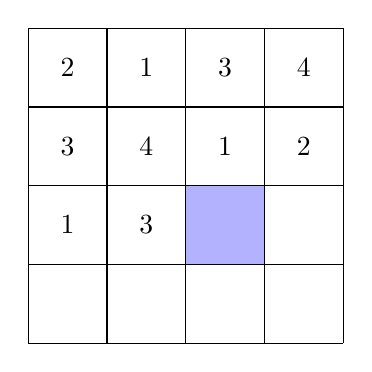
\begin{tikzpicture}
\draw (0,0) grid (4,4);
\node (00) at (0.5,3.5) {2};
\node (01) at (1.5,3.5) {1};
\node (02) at (2.5,3.5) {3};
\node (03) at (3.5,3.5) {4};

\node (10) at (0.5,2.5) {3};
\node (11) at (1.5,2.5) {4};
\node (12) at (2.5,2.5) {1};
\node (13) at (3.5,2.5) {2};

\node (20) at (0.5,1.5) {1};
\node (21) at (1.5,1.5) {3};
\node[draw,fill=blue!30,minimum height=1cm, minimum width=1cm] at (2.5,1.5) {};
\end{tikzpicture}
\bigskip

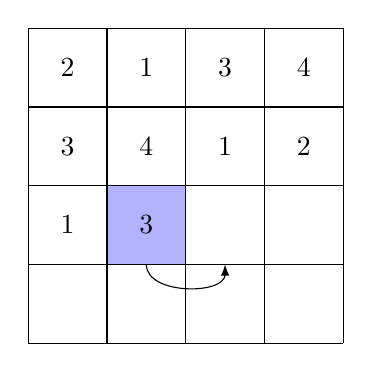
\begin{tikzpicture}
\draw (0,0) grid (4,4);
\node (00) at (0.5,3.5) {2};
\node (01) at (1.5,3.5) {1};
\node (02) at (2.5,3.5) {3};
\node (03) at (3.5,3.5) {4};

\node (10) at (0.5,2.5) {3};
\node (11) at (1.5,2.5) {4};
\node (12) at (2.5,2.5) {1};
\node (13) at (3.5,2.5) {2};

\node (20) at (0.5,1.5) {1};
\node[draw,fill=blue!30,minimum height=1cm, minimum width=1cm] at (1.5,1.5) {3};
\draw[->,>=latex] (1.5,1) to[bend right=90] (2.5,1);
\end{tikzpicture}
\bigskip

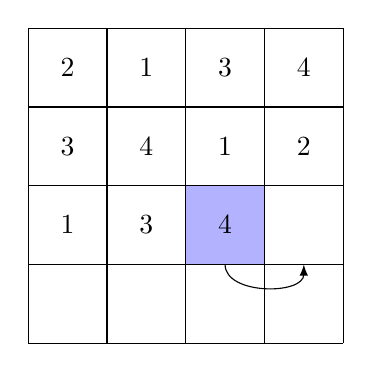
\begin{tikzpicture}
\draw (0,0) grid (4,4);
\node (00) at (0.5,3.5) {2};
\node (01) at (1.5,3.5) {1};
\node (02) at (2.5,3.5) {3};
\node (03) at (3.5,3.5) {4};

\node (10) at (0.5,2.5) {3};
\node (11) at (1.5,2.5) {4};
\node (12) at (2.5,2.5) {1};
\node (13) at (3.5,2.5) {2};

\node (20) at (0.5,1.5) {1};
\node (21) at (1.5,1.5) {3};
\node[draw,fill=blue!30,minimum height=1cm, minimum width=1cm] at (2.5,1.5) {4};
\draw[->,>=latex] (2.5,1) to[bend right=90] (3.5,1);
\end{tikzpicture}
\bigskip

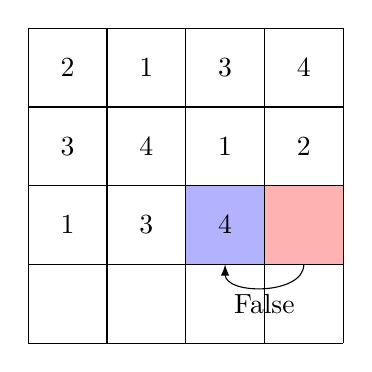
\begin{tikzpicture}
\draw (0,0) grid (4,4);
\node (00) at (0.5,3.5) {2};
\node (01) at (1.5,3.5) {1};
\node (02) at (2.5,3.5) {3};
\node (03) at (3.5,3.5) {4};

\node (10) at (0.5,2.5) {3};
\node (11) at (1.5,2.5) {4};
\node (12) at (2.5,2.5) {1};
\node (13) at (3.5,2.5) {2};

\node (20) at (0.5,1.5) {1};
\node (21) at (1.5,1.5) {3};
\node[draw,fill=blue!30,minimum height=1cm, minimum width=1cm] at (2.5,1.5) {4};
\node[draw,fill=red!30,minimum height=1cm, minimum width=1cm] at (3.5,1.5) {};
\draw[->,>=latex] (3.5,1) to[bend left=90] (2.5,1);
\node at (3,0.5) {False};
\end{tikzpicture}
\bigskip

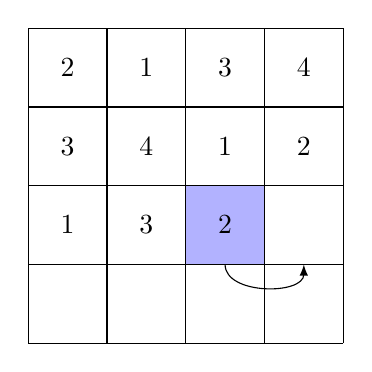
\begin{tikzpicture}
\draw (0,0) grid (4,4);
\node (00) at (0.5,3.5) {2};
\node (01) at (1.5,3.5) {1};
\node (02) at (2.5,3.5) {3};
\node (03) at (3.5,3.5) {4};

\node (10) at (0.5,2.5) {3};
\node (11) at (1.5,2.5) {4};
\node (12) at (2.5,2.5) {1};
\node (13) at (3.5,2.5) {2};

\node (20) at (0.5,1.5) {1};
\node (21) at (1.5,1.5) {3};
\node[draw,fill=blue!30,minimum height=1cm, minimum width=1cm] at (2.5,1.5) {2};
\draw[->,>=latex] (2.5,1) to[bend right=90] (3.5,1);
\end{tikzpicture}
\bigskip

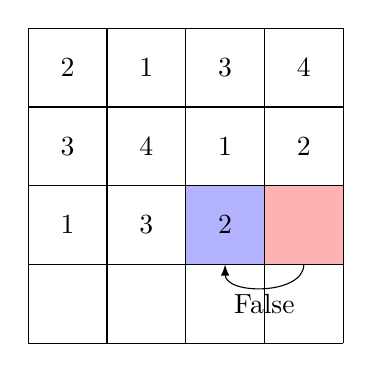
\begin{tikzpicture}
\draw (0,0) grid (4,4);
\node (00) at (0.5,3.5) {2};
\node (01) at (1.5,3.5) {1};
\node (02) at (2.5,3.5) {3};
\node (03) at (3.5,3.5) {4};

\node (10) at (0.5,2.5) {3};
\node (11) at (1.5,2.5) {4};
\node (12) at (2.5,2.5) {1};
\node (13) at (3.5,2.5) {2};

\node (20) at (0.5,1.5) {1};
\node (21) at (1.5,1.5) {3};
\node[draw,fill=blue!30,minimum height=1cm, minimum width=1cm] at (2.5,1.5) {2};
\node[draw,fill=red!30,minimum height=1cm, minimum width=1cm] at (3.5,1.5) {};
\draw[->,>=latex] (3.5,1) to[bend left=90] (2.5,1);
\node at (3,0.5) {False};
\end{tikzpicture}
\bigskip

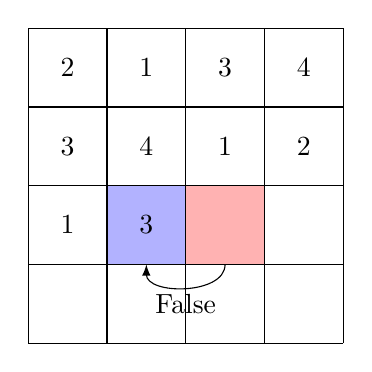
\begin{tikzpicture}
\draw (0,0) grid (4,4);
\node (00) at (0.5,3.5) {2};
\node (01) at (1.5,3.5) {1};
\node (02) at (2.5,3.5) {3};
\node (03) at (3.5,3.5) {4};

\node (10) at (0.5,2.5) {3};
\node (11) at (1.5,2.5) {4};
\node (12) at (2.5,2.5) {1};
\node (13) at (3.5,2.5) {2};

\node (20) at (0.5,1.5) {1};
\node[draw,fill=blue!30,minimum height=1cm, minimum width=1cm]  (21) at (1.5,1.5) {3};
\node[draw,fill=red!30,minimum height=1cm, minimum width=1cm] at (2.5,1.5) {};
\draw[->,>=latex] (2.5,1) to[bend left=90] (1.5,1);
\node at (2,0.5) {False};

\end{tikzpicture}
\bigskip
\end{Form}
\end{document}